\documentclass{sigchi}

% Remove or comment out these two lines for final version
\toappear{ Permission to make digital or hard copies of all or part of
  this work for personal or classroom use is granted without fee
  provided that copies are not made or distributed for profit or
  commercial advantage and that copies bear this notice and the full
  citation on the first page. To copy otherwise, or republish, to post
  on servers or to redistribute to lists, requires prior specific
  permission and/or a fee.

Gamification'13, October 2-4, 2013, Stratford, ON, Canada.

Copyright 2013 ACM 978-1-XXXX-XXXX-X/XX/XX...\$10.00.
}

\pagenumbering{arabic}% Arabic page numbers for submission. 

% Use \toappear{...} to override the default ACM copyright statement (e.g. for preprints).

% Load basic packages
\usepackage{balance}  % to better equalize the last page
\usepackage{graphicx} % for EPS, load graphicx instead
\usepackage{times}    % comment if you want LaTeX's default font
\usepackage{url}      % llt: nicely formatted URLs
\usepackage{paralist} % compact lists


\usepackage{subfigure}
\graphicspath{{figures/}}

% llt: Define a global style for URLs, rather that the default one
\makeatletter
\def\url@leostyle{%
  \@ifundefined{selectfont}{\def\UrlFont{\sf}}{\def\UrlFont{\small\bf\ttfamily}}}
\makeatother
\urlstyle{leo}

% To make various LaTeX processors do the right thing with page size.
\def\pprw{8.5in}
\def\pprh{11in}
\special{papersize=\pprw,\pprh}
\setlength{\paperwidth}{\pprw}
\setlength{\paperheight}{\pprh}
\setlength{\pdfpagewidth}{\pprw}
\setlength{\pdfpageheight}{\pprh}

%% Puts space after macros, unless followed by punctuation
\usepackage{xspace}

%%% Personal macros
%% Tired of typing CO2 so many times, requires xspace package
\newcommand{\COtwo}{CO\ensuremath{_2}\xspace}
%% Hawai`i with okina
\newcommand{\Hawaii}{Hawai`i\xspace}
%% Hawai`ian with okina
\newcommand{\Hawaiian}{Hawai`ian\xspace}
%% Manoa with kahako
\newcommand{\Manoa}{M\=anoa\xspace}

% Make sure hyperref comes last of your loaded packages, 
% to give it a fighting chance of not being over-written, 
% since its job is to redefine many LaTeX commands.
\usepackage[dvips]{hyperref}
\hypersetup{
pdftitle={SGSEAM: Assessing Serious Game Frameworks from a Stakeholder Experience Perspective},
pdfauthor={LaTeX},
pdfkeywords={SIGCHI, proceedings, archival format},
bookmarksnumbered,
pdfstartview={FitH},
colorlinks,
citecolor=black,
filecolor=black,
linkcolor=black,
urlcolor=black,
breaklinks=true,
}

%% Make links to captions point to the figure, not just the caption at bottom
\usepackage[all]{hypcap}

% create a shortcut to typeset table headings
\newcommand\tabhead[1]{\small\textbf{#1}}

%% Since I'm using the LaTeX Makefile that uses dvips, I need this
%% package to make URLs break nicely
\usepackage{breakurl}

% End of preamble. Here it comes the document.
\begin{document}

\title{SGSEAM: Assessing Serious Game Frameworks\\ from a Stakeholder Experience Perspective}

% Note that submissions are blind, so author information should be omitted
%\numberofauthors{5}
%\author{
%  \alignauthor Yongwen Xu, Philip M. Johnson, Carleton A. Moore, Robert S. Brewer, Jordan Takayama\\
%    \affaddr{Department of Information and Computer Sciences}\\
%    \affaddr{University of Hawaii at Manoa}\\
%    \affaddr{Honolulu, HI, USA}\\
%    \email{\{yxu, johnson, cmoore, rbrewer, jktakaya\}@hawaii.edu}\\
%}

\maketitle

\begin{abstract}
% 150 words max
Assessment of serious game frameworks is emerging as an important area of research. 
This paper describes an assessment mechanism called the Serious Game Stakeholder Experience
Assessment Method (SGSEAM). SGSEAM is designed to provide detailed insights into the strengths
and shortcomings of serious game frameworks through a stakeholder perspective based approach.
In this paper, we report on the use of SGSEAM to assess Makahiki, an open source serious game
framework for sustainability. Our results provide useful insights into both Makahiki as a serious game framework and SGSEAM as an assessment method.
\end{abstract}

\keywords{
	serious games; framework assessment; sustainability
}

\category {H.5.m.} {Information Interfaces and Presentation (e.g., HCI)} {Miscellaneous K.8.0.  Personal Computing Games}

%\\
%\textcolor{red}{See: \url{http://www.acm.org/about/class/1998/}
%for more information and the full list of ACM classifiers and descriptors. 
%Mandatory section: On the submission page
%only the classifiers' letter-number combination will need to be entered.}


\terms{
	Serious Game; Assessment; Game Design; Case study.
}

\section{Introduction}

Serious games (games with additional goals beyond just entertainment) have been a topic
of academic research for decades~\cite{Zyda2005}. The recent phenomenon of
gamification~\cite{Deterding2011mt} also calls for evaluation research in areas beyond
traditional entertainment purposes.

One fundamental question in evaluating a serious game or a gamified application is the 
extent to which the game or application achieves its ``serious'' purpose. This is quite different from traditional entertainment games. There is an increasing
focus on the evaluation methodology in the field of serious games ~\cite{Mayer2012233}~\cite{harteveld2010triadic}. These approaches focus on evaluation of a single game, as opposed to a game {\em
  framework}. One of the benefits of 
using a game framework is that, if correctly designed, it will provide useful and
reusable ``building blocks'' with which to develop a variety of serious games. Yet how are we to know if a serious
game framework has been ``correctly designed''?

There exists some assessment tools such as GEQ (Game Engagement Questionnaire)\cite{brockmyer2009development}, QUIS (Questionnaire for User Interaction Satisfaction)\cite{harper1993improving}. We found no prior work concerning comprehensive assessment for 
the particular needs of a serious game framework. To help answer this question, this paper
proposes a method for assessing serious game frameworks, called the Serious Game Stakeholder
Experience Assessment Method (SGSEAM). We consider
SGSEAM as an assessment method instead of an evaluation method. The main purpose of an
evaluation is to "determine the quality of a program by formulating a judgment"
\cite{hurteau2009legitimate}. An assessment, on the other hand, is nonjudgmental. SGSEAM does
not try to judge a framework according to a standard, or to compare one framework against another. Instead, it is used to identify the major
strengths and shortcomings of a framework from the perspectives of major stakeholders. The benefits of 
SGSEAM assessment are for the developers of serious game frameworks to learn from the findings of the assessment.

\section{Serious Game Stakeholder Experience Assessment Method (SGSEAM)}

The goal of SGSEAM is to identify (a) major strengths of a serious game
framework, which aids the community by indicating features of the framework to emulate, and
(b) major shortcomings of the framework, which aids the community by indicating features to avoid.
The target audiences of SGSEAM are the developers of the serious game framework.

The approach that SGSEAM uses is to assess the experiences of various important stakeholders when
they interact with the serious game framework. In the full life cycle of a serious game framework
there are a great variety of potential stakeholders, including:

\begin{compactitem}
\item \emph{Players}: those who participate in the game produced by the framework.
\item \emph{System admins}: those who install and maintain the technological game infrastructure.
\item \emph{Game designers}: those who design the content and game mechanics. They include  content experts, instructional designers, etc.
\item \emph{Game managers}: those who manage the game during the period of game play.
\item \emph{Developers}: those who extend, enhance and debug the game framework.
\item \emph{Community partners}: those who partner with the game
  organizers to help run the game (such as coordinating real-world
  events as part of the game).
\item \emph{Funding organizations}: the organizations who provide
  funding for the game or game framework.
\end{compactitem}

The scope of SGSEAM is to assess serious game frameworks as software infrastructure. While
the overall success of a serious game depends on the individual success of all of these
stakeholders, SGSEAM only assess the experiences of the players, system admins, game designers, game managers, and developers.

SGSEAM employs the concurrent triangulation strategy \cite{creswell2003} of the mixed method of quantitative and qualitative data collection and analysis including instrument and
analytical data recorded by the system such as website logs, user interaction database, as well
as interviews and questionnaire responses.

Similar to "Goal-Question-Metric" (GQM) approach \cite{caldiera1994goal} in
software engineering research, The assessment goals in SGSEAM are to identify the strength and weakness of each identified stakeholders. For each
stakeholder, a set of questions and alternative assessment approaches are
proposed. 

\autoref{fig:overview} provides an overview of the assessment method:

\begin{table}
  \centering
  \begin{tabular}{|c|c|c|}
    \hline
    \multicolumn{1}{|p{0.2\columnwidth}|}{\centering\tabhead{Stakeholder}} &
    \multicolumn{1}{|p{0.35\columnwidth}|}{\centering\tabhead{Assessment Goal}} &
    \multicolumn{1}{|p{0.35\columnwidth}|}{\centering\tabhead{Assessment approaches}} \\
    \hline
    \multicolumn{1}{|p{0.2\columnwidth}|}{Players} &
    \multicolumn{1}{|p{0.35\columnwidth}|}{To what extent does the system affect players?
        To what extent does the system engage players?} &
    \multicolumn{1}{|p{0.35\columnwidth}|}{experimental study, interviews,
                engagement metrics} \\
    \hline
    \multicolumn{1}{|p{0.2\columnwidth}|}{System admins} &
    \multicolumn{1}{|p{0.35\columnwidth}|}{How easy is it to install and maintain the system?} &
    \multicolumn{1}{|p{0.35\columnwidth}|}{experimental study, interviews} \\
    \hline
    \multicolumn{1}{|p{0.2\columnwidth}|}{Game designer} &
    \multicolumn{1}{|p{0.35\columnwidth}|}{How easy is it to design a game?} &
    \multicolumn{1}{|p{0.35\columnwidth}|}{experimental study, system logs, interviews } \\
    \hline
    \multicolumn{1}{|p{0.2\columnwidth}|}{Game managers} &
    \multicolumn{1}{|p{0.35\columnwidth}|}{How easy is it to manage a game?} &
    \multicolumn{1}{|p{0.35\columnwidth}|}{experimental study, system logs, interviews} \\
    \hline
    \multicolumn{1}{|p{0.2\columnwidth}|}{Developers} &
    \multicolumn{1}{|p{0.35\columnwidth}|}{How easy is it to enhance the system?} &
    \multicolumn{1}{|p{0.35\columnwidth}|}{experimental study, interviews} \\
    \hline
  \end{tabular}
  \caption{Overview of SGSEAM}
  \label{fig:overview}
\end{table}

There are usually multiple assessment approaches for a specific question. Different assessment
approaches will have different levels of rigor. In experimental design terms, rigor refers to
external and internal validity. The assessment approaches for a question
can be additive. The more approaches applied, the higher confidence of the assessment.

\section{Case Study of Assessing Makahiki using SGSEAM}

This section presents a case study of how we applied SGSEAM to assess Makahiki, an open source serious game framework for sustainability\cite{csdl2-12-06}. Makahiki is an serious
game framework with the purpose of education and behavioral change regarding energy and water consumption. It can be tailored to the needs of different organizations. Makahiki had been used to create four different Kukui Cup Energy Challenges at the University of Hawaii (UH) in 2011 and 2012, Hawaii Pacific University (HPU) in 2012, and East-West Center (EWC) in 2012. 
The successful creation of several serious game challenges by different organizations
provides evidence that Makahiki framework can be successfully tailored.

Besides the real world usage of Makahiki in the series of Kukui Cup challenges, we
performed in-lab assessment experiments using SGSEAM. Makahiki was used in a serious game
development course in Spring semester of 2013 at the Information and Computer Sciences
Department of the University of Hawaii at Manoa. There were a total of 8 students who
participated in the experiments.  The participants were either senior undergraduates or
graduate students majoring in Computer Science. During the course, the students installed
Makahiki, configured and designed a serious game instance with Makahiki, and finally
developed an enhancement to the Makahiki framework. We asked the students taking the
course to voluntarily participate in the assessment experiments of Makahiki.

\subsection{Player Assessment}

To assess the effectiveness of the framework for designing games that improve player literacy in sustainability, we
conducted two energy literacy surveys, one before the challenge (pre-game) and one after
the challenge (post-game). 24 players completed both surveys. Out of the total 19 energy
literacy questions, the average number of questions answered correctly is 7.54 before the
challenge, and 8.96 after the challenge. This result indicates an 18\% (p=0.056) improvement on the
energy literacy.  We also surveyed non-players as a control condition, and found that
their literacy did not change, indicating that the improvement in player literacy was
indeed due to the game. 

To assess the effectiveness of the framework for designing games that produce positive change in sustainability
behaviors, we recorded and analyzed energy consumption data before, during and after the
challenge.  Before the challenge, an energy usage baseline was established. During the
challenge, compared to the baseline, 12 out of the total 20 teams reduced their energy
consumption, with the highest reduction of 16.1\%. However, 3 teams actually increased
their energy consumption, with the highest increase of 11.7\%. Overall, the average
reduction of the 20 teams was very low---approximately 2\%.

To assess player engagement of the game, we calculated a variety of engagement
metrics. The results are shown in \autoref{fig:makahiki-engagement}:

\begin{table}
  \centering
  \begin{tabular}{|c|c|c|c}
    \hline
    \multicolumn{1}{|p{0.5\columnwidth}|}{\centering\tabhead{Measurement}} &
    \multicolumn{1}{|p{0.1\columnwidth}|}{\centering\tabhead{MIN}} &
    \multicolumn{1}{|p{0.1\columnwidth}|}{\centering\tabhead{AVG}} &
    \multicolumn{1}{|p{0.1\columnwidth}|}{\centering\tabhead{MAX}} \\
    \hline
    \multicolumn{1}{|p{0.5\columnwidth}|}{Participation rate} &
    \multicolumn{1}{|p{0.1\columnwidth}|}{13\%} &
    \multicolumn{1}{|p{0.1\columnwidth}|}{37\%} &
    \multicolumn{1}{|p{0.1\columnwidth}|}{74\%} \\
    \hline
    \multicolumn{1}{|p{0.5\columnwidth}|}{Number of players per day} &
    \multicolumn{1}{|p{0.1\columnwidth}|}{43} &
    \multicolumn{1}{|p{0.1\columnwidth}|}{85} &
    \multicolumn{1}{|p{0.1\columnwidth}|}{147} \\
    \hline
    \multicolumn{1}{|p{0.5\columnwidth}|}{Play time per day} &
    \multicolumn{1}{|p{0.1\columnwidth}|}{1 min} &
    \multicolumn{1}{|p{0.1\columnwidth}|}{27.7 mins} &
    \multicolumn{1}{|p{0.1\columnwidth}|}{8.5 hours} \\
    \hline
    \multicolumn{1}{|p{0.5\columnwidth}|}{submissions per day} &
    \multicolumn{1}{|p{0.1\columnwidth}|}{32} &
    \multicolumn{1}{|p{0.1\columnwidth}|}{266} &
    \multicolumn{1}{|p{0.1\columnwidth}|}{1110} \\
    \hline
    \multicolumn{1}{|p{0.5\columnwidth}|}{social interactions per day} &
    \multicolumn{1}{|p{0.1\columnwidth}|}{51} &
    \multicolumn{1}{|p{0.1\columnwidth}|}{208} &
    \multicolumn{1}{|p{0.1\columnwidth}|}{468} \\
    \hline
    \multicolumn{1}{|p{0.5\columnwidth}|}{website errors per day} &
    \multicolumn{1}{|p{0.1\columnwidth}|}{0} &
    \multicolumn{1}{|p{0.1\columnwidth}|}{0.6} &
    \multicolumn{1}{|p{0.1\columnwidth}|}{4} \\
    \hline
  \end{tabular}
  \caption{Makahiki Engagement Metrics}
  \label{fig:makahiki-engagement}
\end{table}

The average participation rate of this challenge is 37\%, which is good compared to other
sustainability challenges. Over the course of the challenge, an average player spent about
27.7 minutes per day on the website.

In summary, SGSEAM indicates that Makahiki can be successful in achieving
player engagement and literacy improvement. SGSEAM could not provide evidence of positive change in
behavior.

\subsection{System Admin Assessment}

System admin assessment was done using an in-lab experiment.  Students in
the serious game class were tasked with installing the Makahiki system into their local
computers. In order to understand how much time it takes to install Makahiki and what
problems might be encountered, we designed a Google Form explaining the steps required to
install Makahiki. We asked the students to record the time they spent completing each step
and the problems they encountered. We also asked the students to provide feedback about
their installation experiences in the form of blog posts. \cite{csdl2-13-04} describes in detailed
the Google Form that is used in this assessment.

The results from the Google Form responses show that the average total time to successfully install
Makahiki was 1.4 hours, with a maximum time of 2 hours and the minimum time of 0.9 hour.
\autoref{fig:install-time} shows the average time for each installation step.

\begin{figure}
  \center
  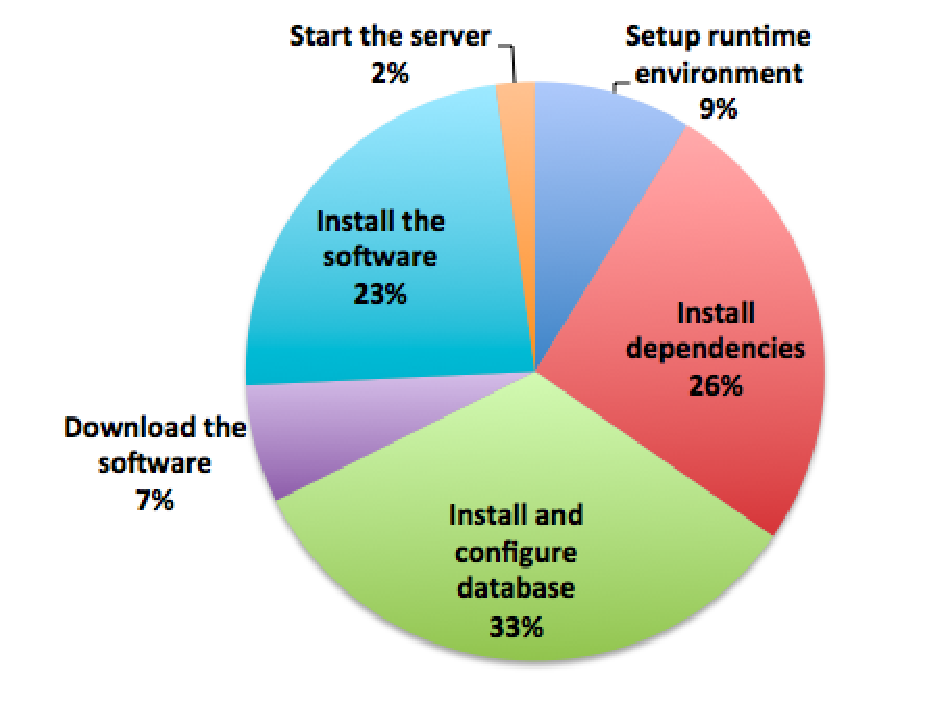
\includegraphics[width=0.6\columnwidth]{install-time}
  \caption{Average time (minutes) for installation steps (n=8)}
  \label{fig:install-time}
\end{figure}

We coded and categorized the descriptive problems reported by the students in both the Google Form
and their blog posts. We identified that the ``Install and configure database'' step has the
longest average time. It is also has the most participant reported problems. This assessment determines the areas for future
improvement are (1) to improve documentation on DB installation, and (2) to improve the install script to automate
more installation tasks.

In summary, SGSEAM identified database installation as a weak point in
installation.  Otherwise, SGSEAM indicates generally positive results regarding
Makahiki with respect to installation. 

\subsection{Game Designer Assessment}

We also used the in-lab experiment to assess the game
designer experience of Makahiki. The students in the
experiment was tasked to design a serious game using the Makahiki framework. We asked the students
to follow specific design steps and record the time required and any problems encountered during
their design process, using a Google Form similar to the one used for the system admin
assessment. In addition, students were asked to provide feedback about their
design experiences in the form of blog posts. \cite{csdl2-13-04} describes in detailed
the Google Form that is used in this assessment.

The game designer assessment was generalized into 7 tasks corresponding to
distinct types of administrative tasks and game design planning. The time for each task is
calculated from the Google Form results.  The most time consuming task
 is "Smart Grid Game Design", which took average 107.9 minutes (56\% of total time) to complete,
 while the least time
  consuming tasks is "Raffle Game Design", which took average 7.9 minutes (7\% of total time)
  to complete.

 We aggregated the problems reported in the feedback of the 8 students that participated in the experiment.
\autoref{fig:makahiki-game-design} shows the result of the analysis:

\begin{table}
  \centering
  \begin{tabular}{|c|c|c|}
    \hline
    \multicolumn{1}{|p{0.7\columnwidth}|}{\centering\tabhead{Problem encountered}} &
    \multicolumn{1}{|p{0.2\columnwidth}|}{\centering\tabhead{Number of participants}} \\
    \hline
    \multicolumn{1}{|p{0.7\columnwidth}|}{Difficulty in understanding predicate system and unlock condition} &
    \multicolumn{1}{|p{0.2\columnwidth}|}{7} \\
    \hline
    \multicolumn{1}{|p{0.7\columnwidth}|}{A bug that prevented users with usernames
containing capital letters from logging in} &
    \multicolumn{1}{|p{0.2\columnwidth}|}{2} \\
    \hline
    \multicolumn{1}{|p{0.7\columnwidth}|}{A bug in the processing of Ajax queries} &
    \multicolumn{1}{|p{0.2\columnwidth}|}{1} \\
    \hline
    \multicolumn{1}{|p{0.7\columnwidth}|}{Difficulty in generating event attendance codes for game activities} &
    \multicolumn{1}{|p{0.2\columnwidth}|}{1} \\
    \hline
  \end{tabular}
  \caption{Makahiki Game Design Analysis, (n=8)}
  \label{fig:makahiki-game-design}
\end{table}

In summary, SGSEAM revealed two shortcomings with Makahiki configuration: ``Smart
Grid Game Design'' and ``Configure Challenge Settings''. Issues encountered in ``Smart Grid Game
Design'' included 1) difficulty and lack of documentation on the predicate system used to define dependencies
between game activities, and 2) difficulty in generating event attendance codes for game activities.
Issues encountered in ``Configure Challenge Settings'' included 1) a bug in the processing of Ajax queries
caused by consecutive clicks on the same interface button, and 2) a bug that prevented users with username
containing capital letters from logging in.

\subsection{Game Manager Assessment}

We used the 2012 Kukui Cup Challenge at the Hawaii Pacific University (HPU) to assess
the game manager experience of Makahiki. We interviewed the
game manager of the HPU Kukui Cup challenge, who is also the game designer of the challenge.
We asked him about his game management experiences using the Makahiki admin
interface.

The interview took place after the challenge and was audio-recorded. We transcribed the
audio recording. The data shows that the game management interface was easy for him to use.
He also discovered a useful feature in the approval interface without
help from the Makahiki support team. The only problem he reported was that after the
competition ended, he discovered that some of the analytics data disappeared. This was
identified by the Makahiki development team as a software bug and has since been fixed.

In summary, SGSEAM uncovered few problems with Makahiki game management using the interview
approach. We realized that the confident level of this assessment approach is low because of
 availability of only one data point. An experimental study approach or perform interviews to
multiple game managers will increase the confidence level of the assessment.

\subsection{Developer Assessment}

We assessed developer experience using an in-lab experiment. One of the class assignments
for the students in the experiment was to develop an enhancement to Makahiki.  This
involved setting up a development environment, following the tutorial to create a ``Hello
world'' widget using Makahiki, and finally, developing an enhancement to extend the
functionality of Makahiki. The students were asked to submit their development source code to the public source code repository and write a blog post to
discuss their efforts to complete the development activity.

All 8 students reported that the first task of creating the simple ``Hello world'' widget
was easy, while the enhancement development was hard. Only one student successfully
completed all 5 required features, while the rest successfully completed 1 or 2
features. The main problem students reported was the lack of documentation for the
development libraries. One student stated in his blog that he decided to choose Makahiki
framework to develop his own serious game because of Makahiki's features and possibility
of reducing development effort by using the framework.

In summary, SGSEAM reveals significant problems with developer efficiency.
Analysis is still ongoing regarding the specific causes of problems and how best to
address them.

\section{Discussion}

We have developed a serious game framework assessment method called Serious Game
Stakeholder Experience Assessment Method (SGSEAM). SGSEAM assesses serious game
frameworks from the perspective of the major stakeholders' experiences. These experiences 
are assessed qualitatively and quantitatively to identify the strengths and
 shortcomings of a serious game framework. We hope that, by using SGSEAM, developers of a serious 
 game framework will gain insights on the areas to improve on, and produce better serious games or gamified applications.

The results of the SGSEAM assessment case study on Makahiki show 
both strengths and
weaknesses in the framework. The assessment has provided actionable
insight into how to improve the framework for system administrators, developers, and game
designers. We now understand Makahiki far better than we did before the application of
SGSEAM.

Our use of SGSEAM also reveals concerns with the assessment method itself.  For certain
stakeholders, we took advantage of a course on serious game design to obtain fairly
detailed quantitative data about, for example, game design assessment.  While we feel
confident of these results, the effort required to collect the data was substantial.  On
the other hand, for other stakeholders such as game managers, we only had access to a
single person who could provide insight from that perspective.  While easier to collect,
the small sample size limits our confident in the data.  We are considering ways to
augment the method with a ``confidence'' value that helps others better interpret the
findings.  

We also realized the needs of applying SGSEAM to other serious game frameworks in order to
understand the effectiveness of SGSEAM.  It is an ongoing research for us.

\section{Acknowledgments}
This research is supported in part by grant IIS-1017126
from the National Science Foundation.

%\textbf{Don't forget
%to acknowledge funding sources as well}, so you don't wind up
%having to correct it later.

% Balancing columns in a ref list is a bit of a pain because you
% either use a hack like flushend or balance, or manually insert
% a column break.  http://www.tex.ac.uk/cgi-bin/texfaq2html?label=balance
% multicols doesn't work because we're already in two-column mode,
% and flushend isn't awesome, so I choose balance.  See this
% for more info: http://cs.brown.edu/system/software/latex/doc/balance.pdf
%
% Note that in a perfect world balance wants to be in the first
% column of the last page.
%
% If balance doesn't work for you, you can remove that and
% hard-code a column break into the bbl file right before you
% submit:
%
% http://stackoverflow.com/questions/2149854/how-to-manually-equalize-columns-
% in-an-ieee-paper-if-using-bibtex
%
% Or, just remove \balance and give up on balancing the last page.
%
\balance

% If you want to use smaller typesetting for the reference list,
% uncomment the following line:
% \small
\bibliographystyle{acm-sigchi}
\bibliography{sustainability,csdl-trs,gamification,yxu}
\end{document}
